\documentclass{llncs}
\usepackage{fullpage}
\usepackage{graphicx}
\usepackage{array}
\usepackage{booktabs}
\usepackage[utf8]{inputenc}
\usepackage{amsmath}
\usepackage{amssymb}
\usepackage{multicol}
\usepackage{eurosym}
\usepackage{cancel}
\usepackage{pgfgantt}
\usepackage{pgfplots}
\usepackage{tikz}
\usetikzlibrary{arrows.meta, positioning}

\begin{document}
\newcolumntype{C}{>{\centering\arraybackslash} m{1.8cm}}
\renewcommand{\figurename}{Diagrama}

\definecolor{Normal}{HTML}{a3b18a}
\definecolor{Critical}{HTML}{ff6b6b}
\definecolor{EdgeNormal}{HTML}{344e41}
\definecolor{EdgeCritical}{HTML}{841818}

\begin{center}
{\huge \textbf{Algoritmo CPM}}

\vspace{1cm}


\textbf{Precedencia de actividades} \\
$A \rightarrow B$ \\
$A \rightarrow C$ \\
$B \rightarrow D$ \\
$C \rightarrow D$ \\

\vspace{0.5cm}

\textbf{Grafo} \\
\vspace{-0.8cm}
\begin{figure}
\centering
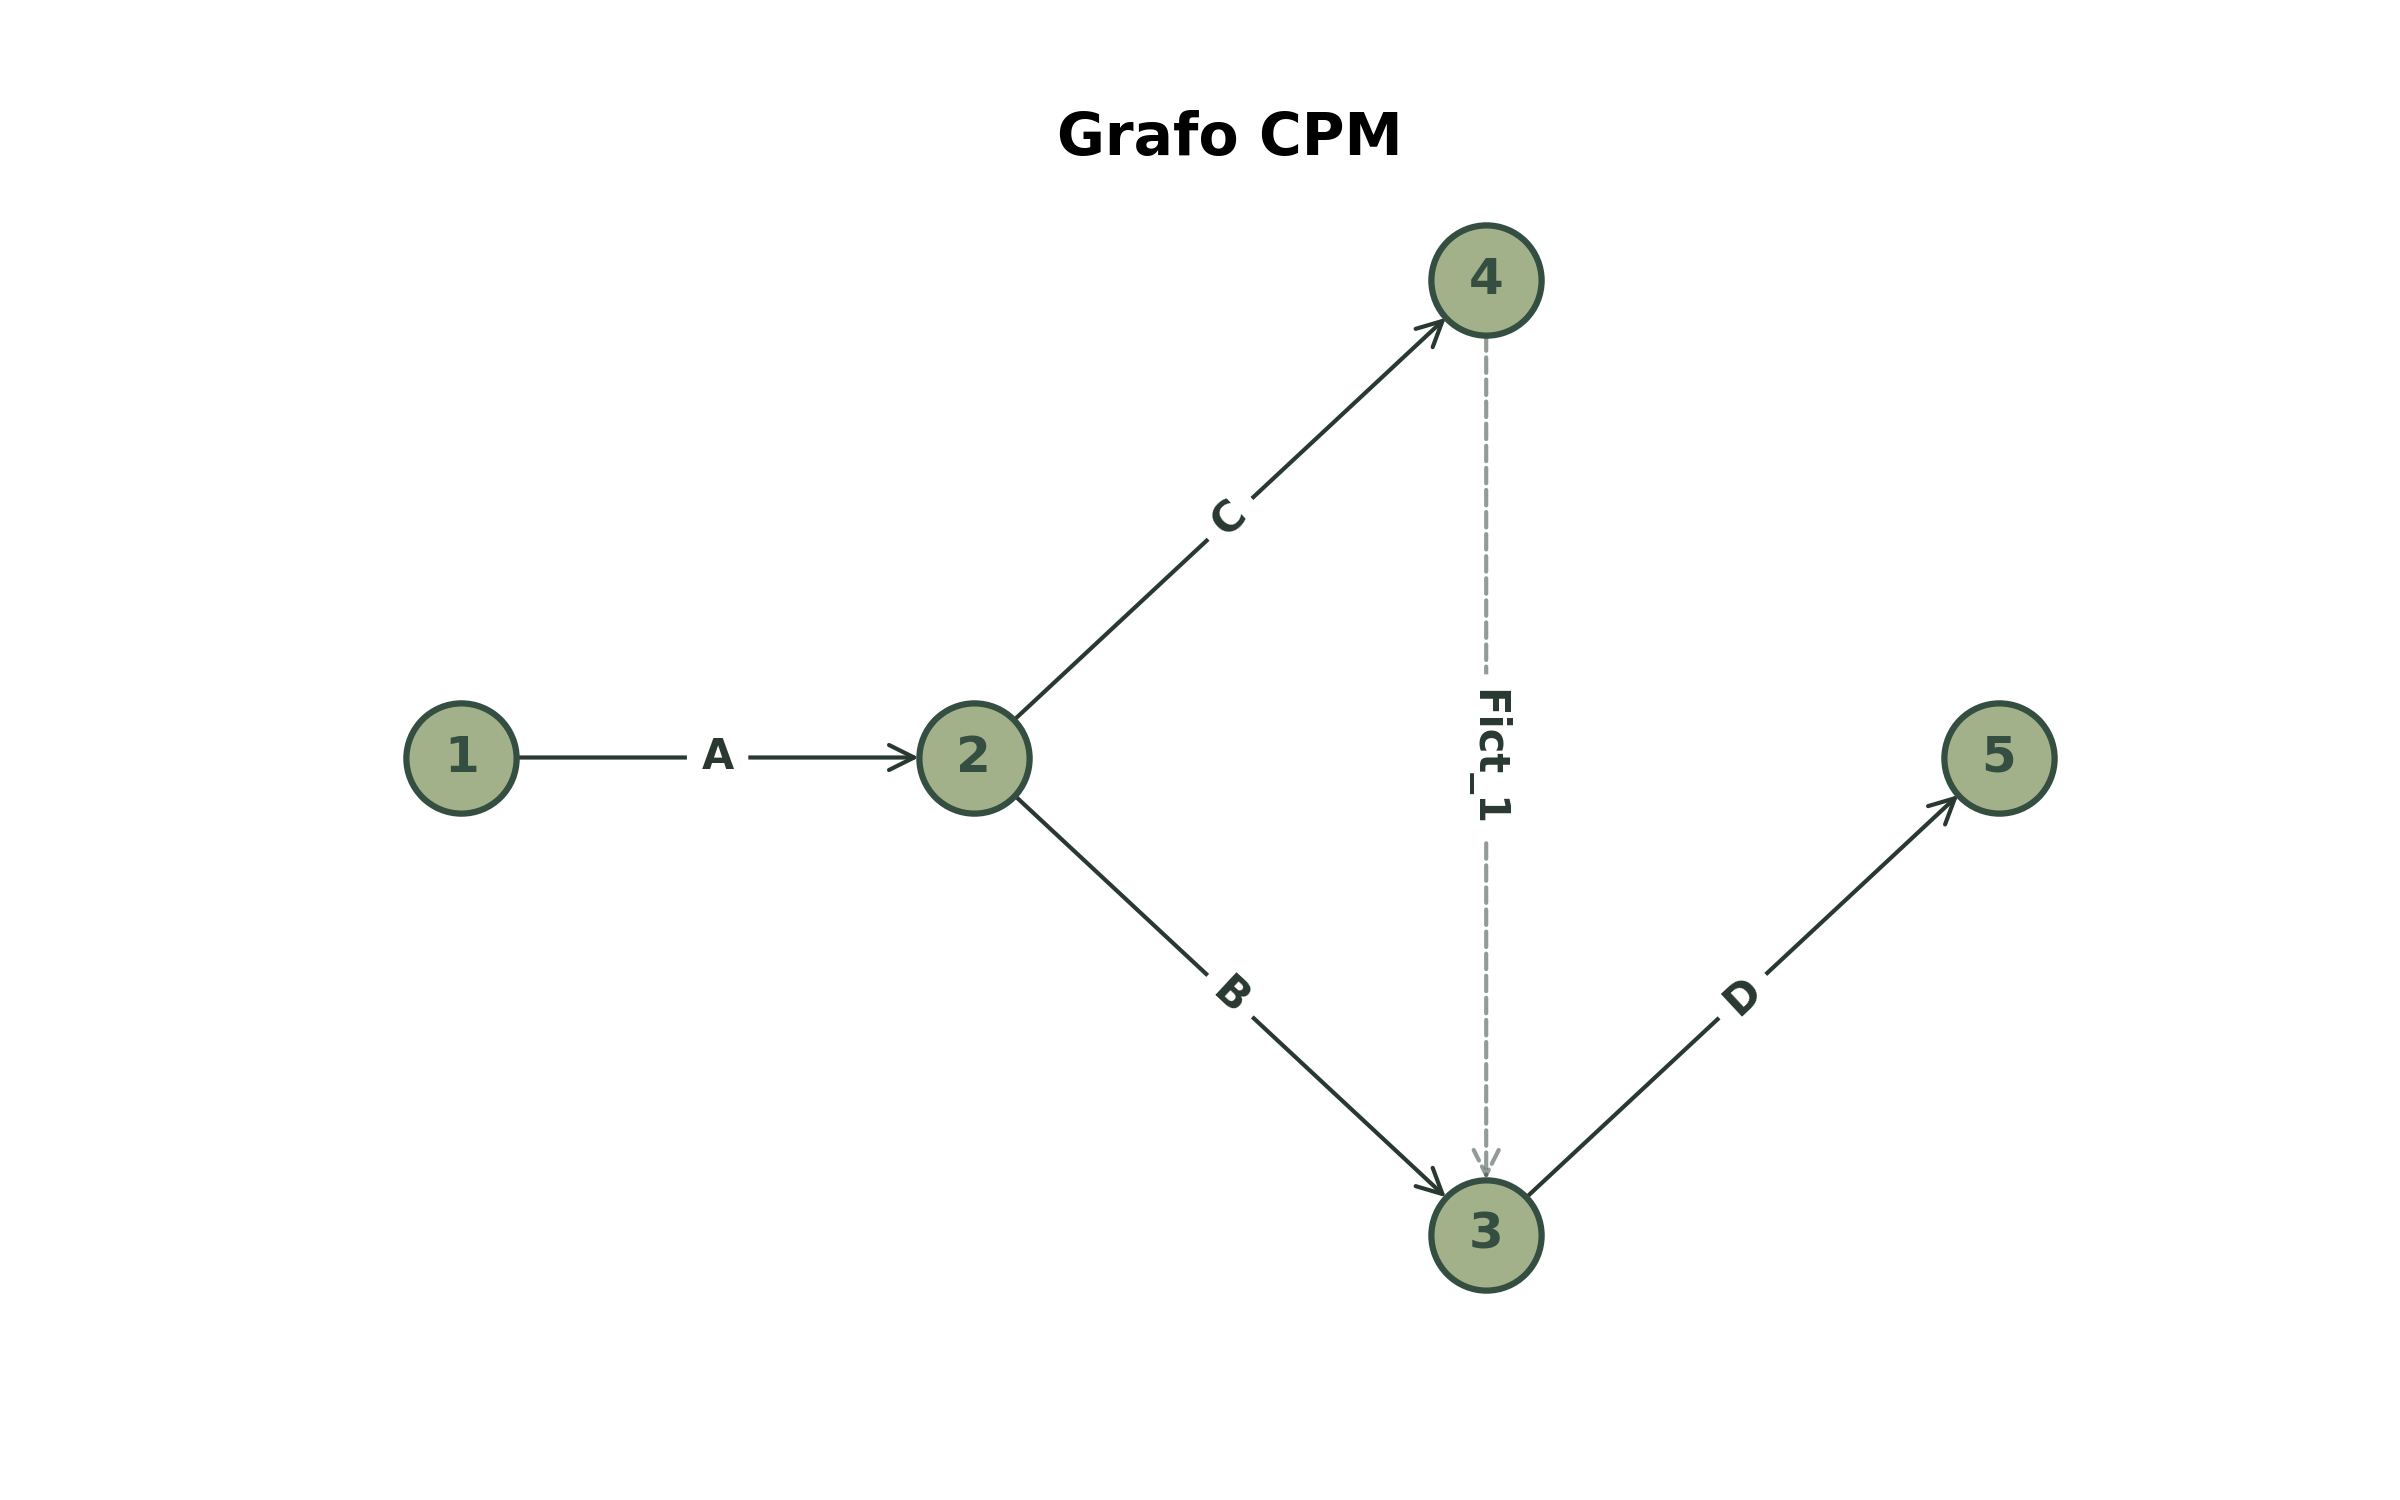
\includegraphics[width=0.95\linewidth]{output_graph.png}
\end{figure}
\end{center}

\newpage

\begin{center}
\textbf{Iteración inicial}
\end{center}

\vspace{0.5cm}

\textbf{Tabla de duraciones y costes}
\begin{table}
\label{tab:tabla1}
\centering
\begin{tabular}{C|CCCCC}
\toprule
Actividad & Duracion (días) & Duración Extrema (días) & Coste (\euro) & Coste Extremo (días) & Slope \\
\midrule
A & 6 & 4 & 600 & 800 & 100.0 \\
B & 8 & 6 & 900 & 1300 & 200.0 \\
C & 5 & 3 & 400 & 600 & 100.0 \\
D & 7 & 5 & 700 & 1100 & 200.0 \\
\bottomrule
\end{tabular}
\end{table} \\

\vspace{0.5cm}

\textbf{Cálculo de Early y Last}
\begin{table}
\label{tab:tabla2}
\centering
\begin{tabular}{C|l}
\toprule
$T_i$ & $Earlies_i$ \\
\midrule
1 & 0 \\
\hline
2 & $E_1 + A = 0 + 6 = 6$ \\
\hline
4 & $E_2 + C = 6 + 5 = 11$ \\
\hline
3 & $\max \left\{ E_2 + B, E_4 + Fict_1 \right\} = \max \left\{ 6 + 8, 11 + 0 \right\} = 14$ \\
\hline
5 & $E_3 + D = 14 + 7 = 21$ \\
\bottomrule
\toprule
$T_i$ & $Lasts_i$ \\
\midrule
1 & $L_2 - A = 6 - 6 = 0$ \\
\hline
2 & $\min \left\{ L_3 - B, L_4 - C \right\} = \min \left\{ 14 - 8, 14 - 5 \right\} = 6$ \\
\hline
4 & $L_3 - Fict_1 = 14 - 0 = 14$ \\
\hline
3 & $L_5 - D = 21 - 7 = 14$ \\
\hline
5 & 21 \\
\bottomrule
\end{tabular}
\end{table} \\

\newpage

\textbf{Cálculo de la holgura y el camino crítico}
\begin{table}
\label{tab:tabla3}
\centering
\begin{tabular}{C|CCCCcC}
\toprule
Tarea & Ruta($i \rightarrow j$) & $Duracion_{ij}$ & $Early_i$ & $Last_j$ & $Holgura_{ij} = Last_j - Early_i - Duracion_{ij}$ & Crítica \\
\midrule
A & $1 \rightarrow 2$ & 6 & 0 & 6 & $H_{ij} = 6 - 0 - 6 = 0$ & Sí \\
B & $2 \rightarrow 3$ & 8 & 6 & 14 & $H_{ij} = 14 - 6 - 8 = 0$ & Sí \\
C & $2 \rightarrow 4$ & 5 & 6 & 14 & $H_{ij} = 14 - 6 - 5 = 3$ & No \\
D & $3 \rightarrow 5$ & 7 & 14 & 21 & $H_{ij} = 21 - 14 - 7 = 0$ & Sí \\
\bottomrule
\end{tabular}
\end{table}

\begin{multicols}{2}
\textbf{Camino crítico:}

A - B - D

\textbf{Duración del proyecto:}

21
\end{multicols}

\vspace{0.5cm}

\textbf{Diagrama de Gantt}
\begin{figure}[h]
\centering
\begin{ganttchart}[vgrid, x unit=0.8cm, y unit title=1cm, y unit chart=0.8cm, bar/.append style={fill=Normal, draw=EdgeNormal, line width=1pt}, bar height=0.6]{0}{21}
\gantttitlelist{0 ,...,21}{1} \\
\ganttbar[bar/.append style={fill=Critical, draw=EdgeCritical, fill opacity=0.5}]{A}{0}{5}
\ganttbar[bar/.append style={fill=Critical, draw=EdgeCritical}]{A}{0}{5} \\
\ganttbar[bar/.append style={fill=Critical, draw=EdgeCritical, fill opacity=0.5}]{B}{6}{13}
\ganttbar[bar/.append style={fill=Critical, draw=EdgeCritical}]{B}{6}{13} \\
\ganttbar[bar/.append style={fill=Normal, draw=EdgeNormal, fill opacity=0.5}]{C}{6}{10}
\ganttbar{C}{6}{10} \\
\ganttbar[bar/.append style={fill=Critical, draw=EdgeCritical, fill opacity=0.5}]{D}{14}{20}
\ganttbar[bar/.append style={fill=Critical, draw=EdgeCritical}]{D}{14}{20} \\
\end{ganttchart}
\end{figure}

\vspace{0.5cm}

\textbf{Coste del proyecto}

A (600\euro) + B (900\euro) + C (400\euro) + D (700\euro) + (0\euro + (150\euro $\cdot$ 21 días)) = 600 + 900 + 400 + 700 + 3150 = 5750\euro

\newpage

\begin{center}
\textbf{Iteración 1}
\end{center}

\vspace{0.5cm}

\textbf{Tabla de duraciones y costes}
\begin{table}
\label{tab:tabla1}
\centering
\begin{tabular}{C|CCCCC}
\toprule
Actividad & Duracion (días) & Duración Extrema (días) & Coste (\euro) & Coste Extremo (días) & Slope \\
\midrule
A & 5 & 4 & 700.0 & 800 & 100.0 \\
B & 8 & 6 & 900 & 1300 & 200.0 \\
C & 5 & 3 & 400 & 600 & 100.0 \\
D & 7 & 5 & 700 & 1100 & 200.0 \\
\bottomrule
\end{tabular}
\end{table} \\

\vspace{0.5cm}

\textbf{Cálculo de Early y Last}
\begin{table}
\label{tab:tabla2}
\centering
\begin{tabular}{C|l}
\toprule
$T_i$ & $Earlies_i$ \\
\midrule
1 & 0 \\
\hline
2 & $E_1 + A = 0 + 5 = 5$ \\
\hline
4 & $E_2 + C = 5 + 5 = 10$ \\
\hline
3 & $\max \left\{ E_2 + B, E_4 + Fict_1 \right\} = \max \left\{ 5 + 8, 10 + 0 \right\} = 13$ \\
\hline
5 & $E_3 + D = 13 + 7 = 20$ \\
\bottomrule
\toprule
$T_i$ & $Lasts_i$ \\
\midrule
1 & $L_2 - A = 5 - 5 = 0$ \\
\hline
2 & $\min \left\{ L_3 - B, L_4 - C \right\} = \min \left\{ 13 - 8, 13 - 5 \right\} = 5$ \\
\hline
4 & $L_3 - Fict_1 = 13 - 0 = 13$ \\
\hline
3 & $L_5 - D = 20 - 7 = 13$ \\
\hline
5 & 20 \\
\bottomrule
\end{tabular}
\end{table} \\

\newpage

\textbf{Cálculo de la holgura y el camino crítico}
\begin{table}
\label{tab:tabla3}
\centering
\begin{tabular}{C|CCCCcC}
\toprule
Tarea & Ruta($i \rightarrow j$) & $Duracion_{ij}$ & $Early_i$ & $Last_j$ & $Holgura_{ij} = Last_j - Early_i - Duracion_{ij}$ & Crítica \\
\midrule
A & $1 \rightarrow 2$ & 5 & 0 & 5 & $H_{ij} = 5 - 0 - 5 = 0$ & Sí \\
B & $2 \rightarrow 3$ & 8 & 5 & 13 & $H_{ij} = 13 - 5 - 8 = 0$ & Sí \\
C & $2 \rightarrow 4$ & 5 & 5 & 13 & $H_{ij} = 13 - 5 - 5 = 3$ & No \\
D & $3 \rightarrow 5$ & 7 & 13 & 20 & $H_{ij} = 20 - 13 - 7 = 0$ & Sí \\
\bottomrule
\end{tabular}
\end{table}

\begin{multicols}{2}
\textbf{Camino crítico:}

A - B - D

\textbf{Duración del proyecto:}

20
\end{multicols}

\vspace{0.5cm}

\textbf{Diagrama de Gantt}
\begin{figure}[h]
\centering
\begin{ganttchart}[vgrid, x unit=0.8cm, y unit title=1cm, y unit chart=0.8cm, bar/.append style={fill=Normal, draw=EdgeNormal, line width=1pt}, bar height=0.6]{0}{21}
\gantttitlelist{0 ,...,21}{1} \\
\ganttbar[bar/.append style={fill=Critical, draw=EdgeCritical, fill opacity=0.5}]{A}{0}{5}
\ganttbar[bar/.append style={fill=Critical, draw=EdgeCritical}]{A}{0}{4} \\
\ganttbar[bar/.append style={fill=Critical, draw=EdgeCritical, fill opacity=0.5}]{B}{5}{12}
\ganttbar[bar/.append style={fill=Critical, draw=EdgeCritical}]{B}{5}{12} \\
\ganttbar[bar/.append style={fill=Normal, draw=EdgeNormal, fill opacity=0.5}]{C}{5}{9}
\ganttbar{C}{5}{9} \\
\ganttbar[bar/.append style={fill=Critical, draw=EdgeCritical, fill opacity=0.5}]{D}{13}{19}
\ganttbar[bar/.append style={fill=Critical, draw=EdgeCritical}]{D}{13}{19} \\
\end{ganttchart}
\end{figure}

\vspace{0.5cm}

\textbf{Coste del proyecto}

A (700.0\euro) + B (900\euro) + C (400\euro) + D (700\euro) + (0\euro + (150\euro $\cdot$ 20 días)) = 700.0 + 900 + 400 + 700 + 3000 = 5700.0\euro

\newpage

\begin{center}
\textbf{Iteración 2}
\end{center}

\vspace{0.5cm}

\textbf{Tabla de duraciones y costes}
\begin{table}
\label{tab:tabla1}
\centering
\begin{tabular}{C|CCCCC}
\toprule
Actividad & Duracion (días) & Duración Extrema (días) & Coste (\euro) & Coste Extremo (días) & Slope \\
\midrule
A & 4 & 4 & 800.0 & 800 & 100.0 \\
B & 8 & 6 & 900 & 1300 & 200.0 \\
C & 5 & 3 & 400 & 600 & 100.0 \\
D & 7 & 5 & 700 & 1100 & 200.0 \\
\bottomrule
\end{tabular}
\end{table} \\

\vspace{0.5cm}

\textbf{Cálculo de Early y Last}
\begin{table}
\label{tab:tabla2}
\centering
\begin{tabular}{C|l}
\toprule
$T_i$ & $Earlies_i$ \\
\midrule
1 & 0 \\
\hline
2 & $E_1 + A = 0 + 4 = 4$ \\
\hline
4 & $E_2 + C = 4 + 5 = 9$ \\
\hline
3 & $\max \left\{ E_2 + B, E_4 + Fict_1 \right\} = \max \left\{ 4 + 8, 9 + 0 \right\} = 12$ \\
\hline
5 & $E_3 + D = 12 + 7 = 19$ \\
\bottomrule
\toprule
$T_i$ & $Lasts_i$ \\
\midrule
1 & $L_2 - A = 4 - 4 = 0$ \\
\hline
2 & $\min \left\{ L_3 - B, L_4 - C \right\} = \min \left\{ 12 - 8, 12 - 5 \right\} = 4$ \\
\hline
4 & $L_3 - Fict_1 = 12 - 0 = 12$ \\
\hline
3 & $L_5 - D = 19 - 7 = 12$ \\
\hline
5 & 19 \\
\bottomrule
\end{tabular}
\end{table} \\

\newpage

\textbf{Cálculo de la holgura y el camino crítico}
\begin{table}
\label{tab:tabla3}
\centering
\begin{tabular}{C|CCCCcC}
\toprule
Tarea & Ruta($i \rightarrow j$) & $Duracion_{ij}$ & $Early_i$ & $Last_j$ & $Holgura_{ij} = Last_j - Early_i - Duracion_{ij}$ & Crítica \\
\midrule
A & $1 \rightarrow 2$ & 4 & 0 & 4 & $H_{ij} = 4 - 0 - 4 = 0$ & Sí \\
B & $2 \rightarrow 3$ & 8 & 4 & 12 & $H_{ij} = 12 - 4 - 8 = 0$ & Sí \\
C & $2 \rightarrow 4$ & 5 & 4 & 12 & $H_{ij} = 12 - 4 - 5 = 3$ & No \\
D & $3 \rightarrow 5$ & 7 & 12 & 19 & $H_{ij} = 19 - 12 - 7 = 0$ & Sí \\
\bottomrule
\end{tabular}
\end{table}

\begin{multicols}{2}
\textbf{Camino crítico:}

A - B - D

\textbf{Duración del proyecto:}

19
\end{multicols}

\vspace{0.5cm}

\textbf{Diagrama de Gantt}
\begin{figure}[h]
\centering
\begin{ganttchart}[vgrid, x unit=0.8cm, y unit title=1cm, y unit chart=0.8cm, bar/.append style={fill=Normal, draw=EdgeNormal, line width=1pt}, bar height=0.6]{0}{21}
\gantttitlelist{0 ,...,21}{1} \\
\ganttbar[bar/.append style={fill=Critical, draw=EdgeCritical, fill opacity=0.5}]{A}{0}{5}
\ganttbar[bar/.append style={fill=Critical, draw=EdgeCritical}]{A}{0}{3} \\
\ganttbar[bar/.append style={fill=Critical, draw=EdgeCritical, fill opacity=0.5}]{B}{4}{11}
\ganttbar[bar/.append style={fill=Critical, draw=EdgeCritical}]{B}{4}{11} \\
\ganttbar[bar/.append style={fill=Normal, draw=EdgeNormal, fill opacity=0.5}]{C}{4}{8}
\ganttbar{C}{4}{8} \\
\ganttbar[bar/.append style={fill=Critical, draw=EdgeCritical, fill opacity=0.5}]{D}{12}{18}
\ganttbar[bar/.append style={fill=Critical, draw=EdgeCritical}]{D}{12}{18} \\
\end{ganttchart}
\end{figure}

\vspace{0.5cm}

\textbf{Coste del proyecto}

A (800.0\euro) + B (900\euro) + C (400\euro) + D (700\euro) + (0\euro + (150\euro $\cdot$ 19 días)) = 800.0 + 900 + 400 + 700 + 2850 = 5650.0\euro

\newpage

\begin{center}
\textbf{Iteración 3}
\end{center}

\vspace{0.5cm}

\textbf{Tabla de duraciones y costes}
\begin{table}
\label{tab:tabla1}
\centering
\begin{tabular}{C|CCCCC}
\toprule
Actividad & Duracion (días) & Duración Extrema (días) & Coste (\euro) & Coste Extremo (días) & Slope \\
\midrule
A & 4 & 4 & 800.0 & 800 & 100.0 \\
B & 7 & 6 & 1100.0 & 1300 & 200.0 \\
C & 5 & 3 & 400 & 600 & 100.0 \\
D & 7 & 5 & 700 & 1100 & 200.0 \\
\bottomrule
\end{tabular}
\end{table} \\

\vspace{0.5cm}

\textbf{Cálculo de Early y Last}
\begin{table}
\label{tab:tabla2}
\centering
\begin{tabular}{C|l}
\toprule
$T_i$ & $Earlies_i$ \\
\midrule
1 & 0 \\
\hline
2 & $E_1 + A = 0 + 4 = 4$ \\
\hline
4 & $E_2 + C = 4 + 5 = 9$ \\
\hline
3 & $\max \left\{ E_2 + B, E_4 + Fict_1 \right\} = \max \left\{ 4 + 7, 9 + 0 \right\} = 11$ \\
\hline
5 & $E_3 + D = 11 + 7 = 18$ \\
\bottomrule
\toprule
$T_i$ & $Lasts_i$ \\
\midrule
1 & $L_2 - A = 4 - 4 = 0$ \\
\hline
2 & $\min \left\{ L_3 - B, L_4 - C \right\} = \min \left\{ 11 - 7, 11 - 5 \right\} = 4$ \\
\hline
4 & $L_3 - Fict_1 = 11 - 0 = 11$ \\
\hline
3 & $L_5 - D = 18 - 7 = 11$ \\
\hline
5 & 18 \\
\bottomrule
\end{tabular}
\end{table} \\

\newpage

\textbf{Cálculo de la holgura y el camino crítico}
\begin{table}
\label{tab:tabla3}
\centering
\begin{tabular}{C|CCCCcC}
\toprule
Tarea & Ruta($i \rightarrow j$) & $Duracion_{ij}$ & $Early_i$ & $Last_j$ & $Holgura_{ij} = Last_j - Early_i - Duracion_{ij}$ & Crítica \\
\midrule
A & $1 \rightarrow 2$ & 4 & 0 & 4 & $H_{ij} = 4 - 0 - 4 = 0$ & Sí \\
B & $2 \rightarrow 3$ & 7 & 4 & 11 & $H_{ij} = 11 - 4 - 7 = 0$ & Sí \\
C & $2 \rightarrow 4$ & 5 & 4 & 11 & $H_{ij} = 11 - 4 - 5 = 2$ & No \\
D & $3 \rightarrow 5$ & 7 & 11 & 18 & $H_{ij} = 18 - 11 - 7 = 0$ & Sí \\
\bottomrule
\end{tabular}
\end{table}

\begin{multicols}{2}
\textbf{Camino crítico:}

A - B - D

\textbf{Duración del proyecto:}

18
\end{multicols}

\vspace{0.5cm}

\textbf{Diagrama de Gantt}
\begin{figure}[h]
\centering
\begin{ganttchart}[vgrid, x unit=0.8cm, y unit title=1cm, y unit chart=0.8cm, bar/.append style={fill=Normal, draw=EdgeNormal, line width=1pt}, bar height=0.6]{0}{21}
\gantttitlelist{0 ,...,21}{1} \\
\ganttbar[bar/.append style={fill=Critical, draw=EdgeCritical, fill opacity=0.5}]{A}{0}{5}
\ganttbar[bar/.append style={fill=Critical, draw=EdgeCritical}]{A}{0}{3} \\
\ganttbar[bar/.append style={fill=Critical, draw=EdgeCritical, fill opacity=0.5}]{B}{4}{11}
\ganttbar[bar/.append style={fill=Critical, draw=EdgeCritical}]{B}{4}{10} \\
\ganttbar[bar/.append style={fill=Normal, draw=EdgeNormal, fill opacity=0.5}]{C}{4}{8}
\ganttbar{C}{4}{8} \\
\ganttbar[bar/.append style={fill=Critical, draw=EdgeCritical, fill opacity=0.5}]{D}{11}{17}
\ganttbar[bar/.append style={fill=Critical, draw=EdgeCritical}]{D}{11}{17} \\
\end{ganttchart}
\end{figure}

\vspace{0.5cm}

\textbf{Coste del proyecto}

A (800.0\euro) + B (1100.0\euro) + C (400\euro) + D (700\euro) + (0\euro + (150\euro $\cdot$ 18 días)) = 800.0 + 1100.0 + 400 + 700 + 2700 = 5700.0\euro

\newpage

\begin{center}
\textbf{Iteración 4}
\end{center}

\vspace{0.5cm}

\textbf{Tabla de duraciones y costes}
\begin{table}
\label{tab:tabla1}
\centering
\begin{tabular}{C|CCCCC}
\toprule
Actividad & Duracion (días) & Duración Extrema (días) & Coste (\euro) & Coste Extremo (días) & Slope \\
\midrule
A & 4 & 4 & 800.0 & 800 & 100.0 \\
B & 6 & 6 & 1300.0 & 1300 & 200.0 \\
C & 5 & 3 & 400 & 600 & 100.0 \\
D & 7 & 5 & 700 & 1100 & 200.0 \\
\bottomrule
\end{tabular}
\end{table} \\

\vspace{0.5cm}

\textbf{Cálculo de Early y Last}
\begin{table}
\label{tab:tabla2}
\centering
\begin{tabular}{C|l}
\toprule
$T_i$ & $Earlies_i$ \\
\midrule
1 & 0 \\
\hline
2 & $E_1 + A = 0 + 4 = 4$ \\
\hline
4 & $E_2 + C = 4 + 5 = 9$ \\
\hline
3 & $\max \left\{ E_2 + B, E_4 + Fict_1 \right\} = \max \left\{ 4 + 6, 9 + 0 \right\} = 10$ \\
\hline
5 & $E_3 + D = 10 + 7 = 17$ \\
\bottomrule
\toprule
$T_i$ & $Lasts_i$ \\
\midrule
1 & $L_2 - A = 4 - 4 = 0$ \\
\hline
2 & $\min \left\{ L_3 - B, L_4 - C \right\} = \min \left\{ 10 - 6, 10 - 5 \right\} = 4$ \\
\hline
4 & $L_3 - Fict_1 = 10 - 0 = 10$ \\
\hline
3 & $L_5 - D = 17 - 7 = 10$ \\
\hline
5 & 17 \\
\bottomrule
\end{tabular}
\end{table} \\

\newpage

\textbf{Cálculo de la holgura y el camino crítico}
\begin{table}
\label{tab:tabla3}
\centering
\begin{tabular}{C|CCCCcC}
\toprule
Tarea & Ruta($i \rightarrow j$) & $Duracion_{ij}$ & $Early_i$ & $Last_j$ & $Holgura_{ij} = Last_j - Early_i - Duracion_{ij}$ & Crítica \\
\midrule
A & $1 \rightarrow 2$ & 4 & 0 & 4 & $H_{ij} = 4 - 0 - 4 = 0$ & Sí \\
B & $2 \rightarrow 3$ & 6 & 4 & 10 & $H_{ij} = 10 - 4 - 6 = 0$ & Sí \\
C & $2 \rightarrow 4$ & 5 & 4 & 10 & $H_{ij} = 10 - 4 - 5 = 1$ & No \\
D & $3 \rightarrow 5$ & 7 & 10 & 17 & $H_{ij} = 17 - 10 - 7 = 0$ & Sí \\
\bottomrule
\end{tabular}
\end{table}

\begin{multicols}{2}
\textbf{Camino crítico:}

A - B - D

\textbf{Duración del proyecto:}

17
\end{multicols}

\vspace{0.5cm}

\textbf{Diagrama de Gantt}
\begin{figure}[h]
\centering
\begin{ganttchart}[vgrid, x unit=0.8cm, y unit title=1cm, y unit chart=0.8cm, bar/.append style={fill=Normal, draw=EdgeNormal, line width=1pt}, bar height=0.6]{0}{21}
\gantttitlelist{0 ,...,21}{1} \\
\ganttbar[bar/.append style={fill=Critical, draw=EdgeCritical, fill opacity=0.5}]{A}{0}{5}
\ganttbar[bar/.append style={fill=Critical, draw=EdgeCritical}]{A}{0}{3} \\
\ganttbar[bar/.append style={fill=Critical, draw=EdgeCritical, fill opacity=0.5}]{B}{4}{11}
\ganttbar[bar/.append style={fill=Critical, draw=EdgeCritical}]{B}{4}{9} \\
\ganttbar[bar/.append style={fill=Normal, draw=EdgeNormal, fill opacity=0.5}]{C}{4}{8}
\ganttbar{C}{4}{8} \\
\ganttbar[bar/.append style={fill=Critical, draw=EdgeCritical, fill opacity=0.5}]{D}{10}{16}
\ganttbar[bar/.append style={fill=Critical, draw=EdgeCritical}]{D}{10}{16} \\
\end{ganttchart}
\end{figure}

\vspace{0.5cm}

\textbf{Coste del proyecto}

A (800.0\euro) + B (1300.0\euro) + C (400\euro) + D (700\euro) + (0\euro + (150\euro $\cdot$ 17 días)) = 800.0 + 1300.0 + 400 + 700 + 2550 = 5750.0\euro

\newpage

\textbf{Curva Coste / Tiempo}
\begin{figure}
\centering
\begin{tikzpicture}
\begin{axis}[title={\textbf{Curva Coste / Tiempo}}, xlabel={Duración (días)}, ylabel={Coste Total (\euro)}, width=10cm, height=7cm, grid=major, grid style={dashed,gray!30}, x dir=reverse]
\addplot[color={Normal}, mark=*, thick, mark options={fill={EdgeNormal}, draw={EdgeNormal}, solid}] coordinates {(21,5750) (20,5700.0) (19,5650.0) (18,5700.0) (17,5750.0) };
\addlegendentry{Coste Total}
\node[coordinate, pin={[align=center]90:{Duración \\ óptima}}] at (axis cs:19,5650.0) {};
\end{axis}
\end{tikzpicture}
\end{figure}
\end{document}